\section{历史研究结果、成本与原 G-A 决策}\label{sec:historical}
\subsection{K1--K4 的工程结果}
\begin{longtable}{L{12mm}L{48mm}L{89mm}}
\caption{截至 2026-09-30 的工程结果与有效解释。}\\
\toprule 工作 & 完成内容 & 有效解释与限制\\\midrule\endfirsthead
\caption[]{（续）}\\
\toprule 工作 & 完成内容 & 有效解释与限制\\\midrule\endhead
K1 & 见证范围与分类前提投递 & 准备与实际执行说明来自测量状态；保留给定场景 a 确认、b 未决控制。\\
K2 & 运行时迁入 \code{runtime/witness/} & 九个迁移模块的 import 归一化文本及 AST 相同；每侧 977 项源码库存、两类 subject 与结果前后相同。\\
K3 & 源码绑定环境从头重建 & 两套 Python 3.12 环境，每侧 141 个依赖版本与 977 项源码绑定一致，未新增读取准入。\\
K4 & E4 共享观察与票数验收 & a 为两张实质票共享一次见证；b 为弃权。E5 用固定票回放，额外实际见证为零。\\
\bottomrule
\end{longtable}

K2 验收中，a 为 \code{CONFIRMED/EXPANDED_OBSERVED}，b 为 \code{UNRESOLVED/LITERAL_OBSERVED}；manifest 唯一变化字段为重建 venv 的 \code{python_executable}。完整 K2 suite 为 2562 passed / 433.32 秒，harness 为 PASS。这些数值属于迁移时的历史验收，不是本次报告重新执行的结果，也不作为新模型进程的 pass stamp。\cite{k2}

这些真实源码 worker 是 developer-scripted 驱动的控制。其工具 provenance 可记录 model-proposed 数据接口，但实验来源仍是给定脚本，不能计为真实模型自主提出成功。

\subsection{M0 与 E-iter 的调用账本}
本节冻结共享授权账本的范围，不包括此前其他实验或文档写作的内部调用。当前工程修复及本报告没有新增项目真实模型 API 请求。

\begin{table}[htbp]
\centering\small
\begin{tabularx}{\textwidth}{L{32mm}r r Y}
\toprule 范围 & 实际请求 & Reported tokens & 观察\\\midrule
M0 阶段 1 & 32 & 191177 & A/B 四格全部弃权；B-a 未完成准备。\\
M0 阶段 2 & 14 & 90153 & 唯一一次 B 两格重跑；实际执行后仍未确认。\\
追加 E-iter & 26 & 166482 & 四格全部弃权，未发生模型驱动的第二场景执行。\\
\midrule
本轮共享账本累计 & 72 & 447812 & 低于 210 请求、2500000 reported tokens 上限。\\
\bottomrule
\end{tabularx}
\caption{统计范围限定为 M0 与追加 E-iter 的共享授权账本。此前历史实验在各自档案中分别保留。}
\end{table}

\begin{table}[htbp]
\centering\small
\begin{tabularx}{\textwidth}{L{37mm}r r L{18mm}Y}
\toprule E-iter 格子 & 请求 & Tokens & 执行次数 & 人工复核的主要缺口\\\midrule
开发见证 a & 6 & 36234 & 1 & F3，场景选择不满足目标见证条件。\\
开发见证 b & 7 & 44985 & 1 & 同一分支与记录前缀缺口；最终弃权。\\
近迁移 callback a & 7 & 45465 & 1 & F4，临时目录不可用，尚未到进程边界。\\
近迁移 callback b & 6 & 39798 & 1 & 同一隔离/临时目录限制。\\
\bottomrule
\end{tabularx}
\caption{E-iter 四格结果。运行标识分别对应 hp003\_a/b 与 hp004\_a/b；后一对为 entry-00390 的近迁移。}
\end{table}

E-iter 的 26 次返回模型 ID 全部为 \code{deepseek-flash}，每次响应具有 usage，原始日志与独立审计一致。真实调用前新进程门禁为 2556 passed / 390.51 秒。每格只有一次物理场景；两份原始 VULNERABLE/UNRESOLVED 提案被准入拒绝，最终四格均 ABSTAIN。固定侧没有 SAFE、producer CONFIRMED 或已准入 VULNERABLE。\cite{eiter}

开发 a/b 场景选择仍落入不同于目标见证的分支，完整紧凑响应已到达模型，后续动作没有形成第二场景尝试。callback 两格在目标候选帧前被隔离环境的临时目录创建阻断，应归因基础设施 F4，不能计成场景选择能力失败或补丁安全。

\begin{figure}[htbp]\centering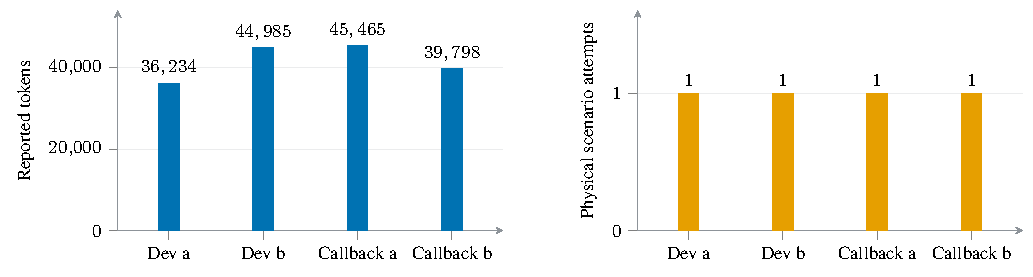
\includegraphics[width=\textwidth]{figures/eiter_cells.pdf}
\caption{E-iter 四格 token 与物理场景次数。每格一个物理场景，四格均 ABSTAIN；配对/同 advisory 数据不构成四个独立仓库样本。}\label{fig:eiter}
\end{figure}

\subsection{失败分类与归因规则}
\begin{table}[htbp]
\centering\small
\begin{tabularx}{\textwidth}{L{11mm}Y}
\toprule 类别 & 预登记解释\\\midrule
F1 & 未调用见证工具，或未走完准备/工具协议。\\
F2 & 场景假设多次被输入 schema 拒绝。\\
F3 & 场景被接受但不足以形成所需见证；必须列出实际缺口。\\
F4 & 见证基础设施、隔离、资源或超时问题。\\
F5 & 见证已确认，但 agent 的最终判定未接纳对应正向证据。\\
F6 & 局部或累计预算耗尽。\\
\bottomrule
\end{tabularx}
\caption{M0 失败分类。自动诊断与人工复核分别保留，类别可以具有伴随因素。}
\end{table}

阶段 1 B-a 的主因是 F1；阶段 2 B-a 主因为 F3，局部 F6 伴随。E-iter 并没有完成模型自主迭代。离线脚本证明工具和原预算可以容纳两个不同场景，不证明真实模型会利用这一能力；提示、协议和投递共同变化的一轮探索也不能隔离预算的因果作用。

\subsection{近迁移、外部样本与 G-A}
3a 的 callback 与原开发样本来自同一 advisory，只是入口近迁移，不是外部项目迁移。离线正确脚本也在临时目录创建处失败，因此 M0 原 3a 的模型运行未满足前置条件；追加 E-iter 包含这两格来自单独授权，不追溯修改原阶段规则。

3b 按预登记顺序冻结前 15 条公告，没有继续从第 16 条挑选。唯一符合源码路径标准的暂定外部候选缺少对应源码版本的目标原生扩展，环境标准未满足，合格外部对数为 0；没有新增 v7、脚本确认或该阶段模型请求。该事实描述当前环境准备能力，没有证明该源码不可构建。

正式 G-A 使用合取条件
\begin{equation}
G\!A=\bigl(\text{原 M0 的 B-a 自主成功}\bigr)
\land\bigl(\text{3b 至少一对外部迁移成功}\bigr).
\end{equation}
两项都不满足，故 G-A = NO。developer-scripted 控制、3a 近迁移和追加 E-iter 不参与救回原门槛。K5--K8 未启动；未使用预算也不构成重新启动这些工作的授权。\cite{gate}


\subsection{其他历史资料的当前解释}
项目还保留 OWASP Java、VulnGym 源码检索、synthetic/V 基线、开发配对完整矩阵与 Jev 分流记录。当前状态页明确将其作为写作时快照，不作为修后源码的成绩。早期部分 fixture 曾将权限模式误声明为竞态、将源码字符串形状作为授权证明，或依赖 expected-role 过滤；仅凭旧标签计分无法满足现行性质与范围契约。本文没有重审这些整批请求，不把旧正确率并入当前结果，也不把 72 请求写成项目从创建以来的总用量。\citep{status,contract}

\subsection{历史成本的描述性分析}
三个阶段的请求和 token 分别占总量的不同份额。M0 阶段 1 使用 32/72 请求（44.44\%）和 191177/447812 tokens（42.69\%）；阶段 2 为 14/72（19.44\%）和 90153/447812（20.13\%）；E-iter 为 26/72（36.11\%）和 166482/447812（37.18\%）。这是投入分配，不是各阶段的信息价值测量。

\begin{figure}[htbp]\centering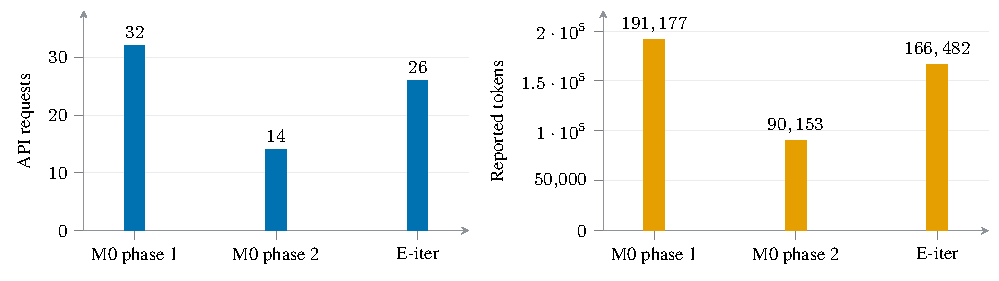
\includegraphics[width=\textwidth]{figures/historical_usage.pdf}
\caption{共享历史账本分阶段用量。Reported tokens 是 provider 响应中的计数，与观察字节预算分开；请求响应解析失败也应保留用量。}\label{fig:usage}
\end{figure}

平均每个实际请求为 \AvgTokensPerRequest\ reported tokens，混合 planner、循环、输入和输出，不能当作一次固定任务的标准成本。E-iter 四格 tokens 均值 41620.5，范围 36234--45465，样本标准差 4413.46；最大/最小约 1.25。这四格每格均一次物理场景，显示 token 数与场景尝试数不是同一个量。相同或更高 token 投入并没有在本轮产生自主确认，但没有匹配对照可估计 token 增量的因果效果。

\begin{figure}[htbp]\centering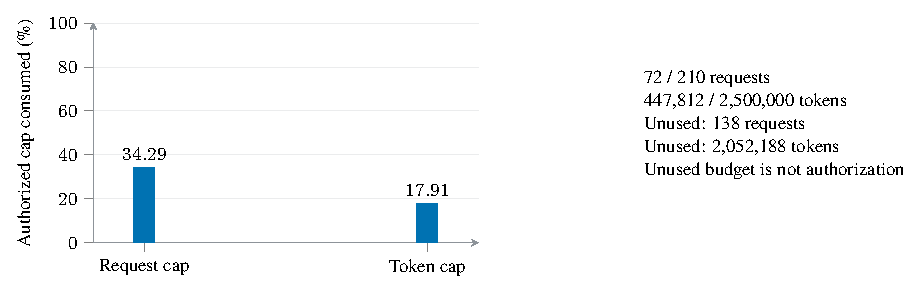
\includegraphics[width=\textwidth]{figures/budget_utilization.pdf}
\caption{历史授权上限的使用比例。请求使用 34.29\%，tokens 使用 17.91\%；余额只是旧账本数值，不授权新实验。}
\end{figure}

余下 138 请求与 2052188 tokens 不改变 G-A，也不等于当前可以再次调用。所有返回模型 ID 以原始响应为准，未知 usage 不能补为零。未提供完整历史价格配置和账单，本文不将 reported tokens 换算成货币费用。
